\documentclass[10pt]{article}
\usepackage{blindtext}
\usepackage{graphicx}
\usepackage{multirow}
\usepackage{amsmath}

\newtheorem{problem}{Problem}

\begin{document}

\title{Efficient Selection of Optimal Time Points Over Biological Time-Series Data}
\date{}

\maketitle

\section{Methods}

\subsection{Problem statement}
Our goal is to identify a (small) subset of time points that can be
used to accurately reconstruct the expression trajectory for {\em
all} genes or other molecules being profiled. We assume that we can
efficiently and cheaply obtain a dense sample for the expression of
a very small subset of representative genes (here we use nanostring
to profile less than $0.5\%$ of all genes) and attempt to use this
subset to determine optimal sampling points for the entire set of
genes.

Formally, let $G$ be the set of genes we have profiled in our dense
sample, $T = \{t_{1}, t_{2}, \ldots, t_{T}\}$ be the set of all
sampled time points. We assume that for each time point we have $R$
repeats for all genes. We denote by $e_{gt}^{r}$ be the expression
value for gene $g \in G$ at time $t \in T$ in the $r$'th repeat for
that time point. We define $D_{g} = \{e_{gt}^{r}\,,\, t \in T, r \in
R$ as the complete data for gene $g$ over all replicates and time
points $T$.

To constrain the set of points we select we assume that we have a
predefined budget $k$ for the maximum number of time points we can
sample in the complete experiment (i.e. for profiling all genes,
miRNAs, epigenetic marks etc. using high throughput seq
experiments). We are interested in selecting $k$ time points from
$T$ which, when using only the data collected at these $k$ points,
minimizes the prediction error for the expression values of the
unused points. To evaluate such a selection, we use the selected
values to obtain a smoothing splines~\cite{deboor, bar2003,
wahba1990} function for each gene and compare the predicted values
based on the spline to the measured value for the non-selected
points to determine the error. In our problem, $t_{1}$ and $t_{T}$
define the first and end points, so they are always selected. The
rest of the points are selected to maximize the following
objective~\ref{prob:prob1}:
%
\begin{problem}\label{prob:prob1}
Given $D_{g}$ for genes $g \in G$, the number of desired time points
$k$ identify a subset of $k-2$ time points in $T \setminus \{t_{1},
t_{T}\}$ which minimizes the prediction error for the expression
values of all genes in the remaining time points.
\end{problem}


\subsection{Spline assignments}

Before discussing the actual procedure we use to select the set of
time points, we discuss the method we use to assign splines based on
a selected subset of point $k$ for each gene. There are two issues
that needs to be resolved when assigning such smoothing splines: 1.
The number of knots (control points) and 2. their spacing. Past
approaches for using splines to model time series gene expression
data have usually used the same number of control points for all
genes regardless of their trajectories~\cite{bar2012, singh2005} and mostly employed uniform
knot placements. However, since our method needs to be able to adapt
to any size of $k$ as defined above, we select them indirectly through
regularization parameter of the fitted smoothing spline where number
of knots will be increased until the smoothing condition is
satisfied. In contrast to the existing methods, we also select knots when fitting a smoothing spline.

\subsection{Iterative process to select points}\label{sec:mainalgo}

Because of the highly combinatorial nature of the time points, selection problem we rely on a greedy iterative process to select
the optimal points as shown in Figure ~\ref{fig:algo}.

There are three key steps in this algorithm which we discuss in
detail below.

\begin{itemize}
\item {\em Selecting the initial set of points:} When using an iterative algorithm to solve non convex problems with several local minima,
a key issue is the appropriate selection of the initial solution
set~\cite{kmeans, mixture}. We have tested a number
of methods for performing such initializations. The simplest method
we tried is to uniformly select a subset of the points (so if
$k=T/4$ we use each 4th point). Another method we tested is to partition the set
of all time points $T$ into $k-1$ intervals of almost equal size by
dynamic programming. Then, it uses $k$ interval boundaries including
$t_{1}$ and $t_{T}$ as initial solution. Finally, we tested a
method that relies on the changes between consecutive time points to
select the most important ones for our initial set. Specifically,
for this we sort all points except $t_{1}$ and $t_{T}$ by average
absolute difference with respect to its predecessor time points by
computing:
%
\begin{equation}
m_{t_{i}} = \frac{\sum_{g \in G} \sum_{d \in D}\,|e_{g t_{i-1}} -
e_{g t_{i}}|}{2 \sum_{g \in G} |D_{g}|}
\end{equation}
where $g t_{i}$ is the average or median expression for gene $g$ at
time $t$. We then select the $k-2$ points with maximum $m_{t_{i}}$
as the initial solution.

\item After selecting the initial set, we begin the iterative process of refining the subset of selected points.
In this step we repeat the following analysis in each iteration. We
exhaustively remove all points from the existing solution (one at a
time) and replace it with all points that were not in the selected
set (again, one at a time). For each pair of such point, we compute
the error resulting from the change (using the splines computed
based on the current set of points evaluated on the left out time
points), and determine if the new point reduces the error or not.
Formally, let $C_n$ be set of points for iteration $n$ We are
interested in finding a point pair $(t_{a} \in C_n, t_{b} \in T
\setminus C_n)$
which minimizes the following error for the next iteration $C_{n+} =
C_n \setminus \{t_{a}\} \cup \{t_{b}\}$:
%
\begin{equation}
\textit{error} = \frac{\sum_{g \in G} \sum_{d \in D}\, \sum_{t \in
    T \setminus C_{n+1}}|\hat{e}_{gt} - e_{gt}^{d}|}{\sum_{g \in G}
  \sum_{d \in D} \sum_{t \in
    T \setminus C_{n}} |\hat{e}_{gt} - e_{gt}^{d}|}
\end{equation}
%
where $\hat{e}_{gt}$ is our spline based estimate of the expression
of gene $g$ at time $t$. If there are pairs which leads to an error
of less than $1$ in the above function, we select the best (lowest
error) and continue the iterative process. Otherwise we terminate
the process and output $C_n$ as the optimal solution. Note that this
greedy process is guaranteed to converge to a (local) minima since
the number of time points is finite.

\begin{figure}
\centering
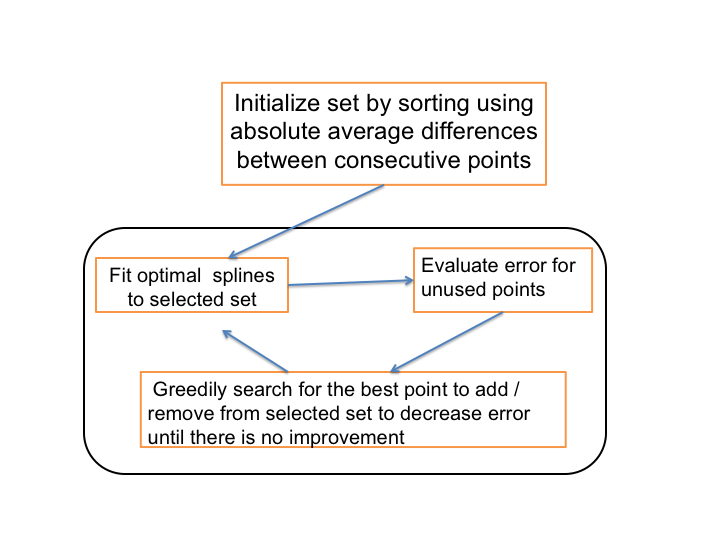
\includegraphics[scale=0.4]{algo.png}
\caption{Summary of our Method}
\label{fig:algo}
\end{figure}

\item Third key step of our approach is fitting smoothing spline to
  gene independently for selected subset of time points. Smoothing
  splines are capable of modeling arbitrary nonlinear shapes as well
  as not having the problem such as Runge's phenomenon seen in other
  fitting methods such as polynomial regression. Smoothing splines
  perform quite well in preventing overfitting~\cite{wahba1990}. Let
  $R = \{(t, y_{t}),\, t \in C\}$, and $\mu$ be the spline we are interested in fitting, smoothing spline
  can be found by the following optimization problem which minimizes
  regularized squared error:
%
\begin{equation}
min \sum_{(t, y_{t}) \in R} \,(y_{t} - \mu(t))^{2} + \lambda \int_{0}^{T_{max}} (\mu^{''}(x))^{2}
\end{equation}
%
where $\lambda$ is the regularization parameter which prevents overfitting. We have estimated regularization parameter by leave one
out cross validation in our experiments. $\lambda$ also affects the number of knots selected. 

\end{itemize}


\subsection{Individual vs. Cluster based Evaluation}\label{sec:clusteval}

In section~\ref{sec:mainalgo}, we assume that error of each
gene has same contribution to the overall error. However, this assumption ignores the
fact that expression of genes are correlated with the expression of other genes. To take the
correlation between genes into account, we have also performed cluster
based evaluation of genes where we analyzed the error by weighting each gene in terms of inverse of the numbers of
genes in the cluster it belongs. This scheme ensures that each cluster
contributes equally to the resulting error rather than each gene. We find clusters by k-means
clustering algorithm over time series-data as well as over a vector of
randomly sampled time points on fitted spline~\cite{bishop2006}. We use Bayesian Information Criterion~(BIC) to
determine the optimal number of clusters~\cite{bic}.

\section{Results}


\bibliographystyle{plain}
\bibliography{expressbib}


\end{document}
